\documentclass[t,aspectratio=169]{beamer}
\usetheme[progressbar=frametitle]{metropolis}
\usefonttheme{professionalfonts}
\usepackage{appendixnumberbeamer}

\usepackage{booktabs}
\usepackage[scale=2]{ccicons}

\usepackage{graphics,graphicx,amssymb,amsmath,pgf,comment,hyperref,multicol}
%\usepackage[xcolor=pst]{pstricks}
\usepackage{array}
\usepackage{pgfshade}
\usepackage[round]{natbib}
\usepackage[absolute,overlay]{textpos}
\usepackage{pifont}
\usepackage{dcolumn}
\usepackage{textpos}
\usepackage{color}					
\usepackage{xcolor,colortbl}
\usepackage{tikz}
\usepackage{bbm}
\usepackage{curves}
\usepackage{mathtools}
\usepackage{times}
\usepackage{verbatim}
\usetikzlibrary{snakes,arrows,shapes,positioning}
\def\augie{\fontencoding{T1}\fontfamily{augie}\selectfont}

\usepackage{pgfplots}
\usepgfplotslibrary{dateplot}

\usepackage{xspace}
\newcommand{\themename}{\textbf{\textsc{metropolis}}\xspace}

\setbeamertemplate{caption}{\raggedright\insertcaption\par}
\usetikzlibrary{calc,decorations.pathmorphing,patterns}
\pgfdeclaredecoration{penciline}{initial}{
    \state{initial}[width=+\pgfdecoratedinputsegmentremainingdistance,
    auto corner on length=1mm,]{
        \pgfpathcurveto%
        {% From
            \pgfqpoint{\pgfdecoratedinputsegmentremainingdistance}
                      {\pgfdecorationsegmentamplitude}
        }
        {%  Control 1
        \pgfmathrand
        \pgfpointadd{\pgfqpoint{\pgfdecoratedinputsegmentremainingdistance}{0pt}}
                    {\pgfqpoint{-\pgfdecorationsegmentaspect
                     \pgfdecoratedinputsegmentremainingdistance}%
                               {\pgfmathresult\pgfdecorationsegmentamplitude}
                    }
        }
        {%TO
        \pgfpointadd{\pgfpointdecoratedinputsegmentlast}{\pgfpoint{1pt}{1pt}}
        }
    }
    \state{final}{}
}


\title{The Price of Specialization in Health Care: Evidence from Children's Hospitals}
\date{}
\author{\textbf{Ian McCarthy} \& Mehul Raval}
\institute{October 7, 2019}

\begin{document}
\tikzstyle{every picture}+=[remember picture]
\everymath{\displaystyle}

\maketitle

\section{Background on Specialty Hospitals}

\begin{frame}{What is a Specialty Hospital?}
    \onslide<1->{
        Hospitals that ``tend to focus on patients with specific medical conditions or who need surgical procedures'' (GAO, 2003)
    }
    \onslide<2->{
    \vspace{.1in}
    \begin{multicols}{2}
        \textbf{Medical conditions}
        \begin{itemize}
            \item Children's hospitals
            \item Rehabilitation centers
            \item Cancer centers
            \item Long-term care (not SNFs)
        \end{itemize}
        \textbf{Surgical procedures}
        \begin{itemize}
            \item Cardiac hospitals
            \item Orthopedic hospitals
            \item Surgery centers
            \item[\vspace{\fill}]
        \end{itemize}
    \end{multicols}
    }
\end{frame}

\begin{frame}[fragile]{Growth of Specialty Hospitals}
    %Number of specialty hospitals
    \begin{center}
    \begin{tikzpicture}
    \pgfmathsetlengthmacro\MajorTickLength{
      \pgfkeysvalueof{/pgfplots/major tick length} * 0.5
    }
    \begin{axis}[
        color=black,
        axis lines*=left,
        width=4in,
        height=3in,
        %bar width=6pt,
        %ybar,
        enlargelimits=0.01,
        ylabel={Number of Hospitals},
        symbolic x coords={2008,2009,2010,2011,2012,2013,2014,2015},
        xtick=data,
        ytick={20,40,60,80,100,120},
        ymin=0,
        ymax=120,
        %nodes near coords,
        %every node near coord/.style={/pgf/number format/precision=0},
        %every node near coord/.append style={font=\tiny},
        %nodes near coords align={vertical},
        %nodes/.style={font=\footnotesize}
    ]
       \addplot[color=blue, thin] coordinates {
        (2008,44)
        (2009,47)
        (2010,46)
        (2011,51)
        (2012,56)
        (2013,51)
        (2014,68)
        (2015,61)
        }
        node[midway,below] {\footnotesize{Cardiac}}
        ;
       \only<2-3>{
       \addplot[color=black, dashed] coordinates {
        (2008,48)
        (2009,54)
        (2010,59)
        (2011,75)
        (2012,80)
        (2013,74)
        (2014,90)
        (2015,85)
        }
        node[midway,below] {\footnotesize{Ortho}}
        ;
       }
       \only<3>{
       \addplot[color=red, dotted] coordinates {
        (2008,62)
        (2009,68)
        (2010,69)
        (2011,84)
        (2012,82)
        (2013,82)
        (2014,100)
        (2015,86)
        }
        node[midway,above] {\footnotesize{Surgical}}
        ;
       }
       \end{axis}
    \end{tikzpicture}
    \end{center}
\end{frame}

\begin{frame}{Concerns about Specialty Hospitals}
    \only<1>{
        \footnotesize
        \begin{itemize}
            \setlength{\itemindent}{1.2em}
            \item[April 2003] Initial study of the prevalence and effects (GAO)
            \item[October 2003] Supplemental study of relationship with certificate of need requirements (GAO)
            \item[March 2004] Moratorium on self-referrals for physician-owned specialty hospitals (MMA 2003)
            \item[May 2005] Report on growth of physician-owned specialty hospitals (GAO)
            \item[May 2005] Reports on effects of physician-owned specialty hospitals to Congress (HHS and MedPAC)
            \item[April 2006] Report on effects of physician-owned specialty hospitals on general hospitals (GAO)
            \item[April 2006] Supplemental testimony to Congress (MedPAC)
            \item[August 2006] Final report to Congress (HHS, as part of Deficit Reduction Act)
        \end{itemize}
        \normalsize
    }
    \only<2>{
        Primary concerns relate to:
        \begin{itemize}
            \item ``Cream-skimming'' of profitable patients (seems to happen)
            \item Self-referrals driven by financial incentives of physician-ownership (small, if any, effect)
            \item Foreclosure of general hospitals (no effects)
        \end{itemize}
    }
    \only<3>{
        Specialty hospitals may also negotiate higher prices without any quality improvements due to:
        \begin{itemize}
            \item Higher costs due to lack of scale
            \item Better accommodations/amenities
            \item Spillover from other specialized services (higher WTP from insurers)
            \item Product differentiation via specialization, real or perceived (Seim, 2006 RAND; Kalra and Li, 2008 Management Science)
        \end{itemize}
    }
\end{frame}

\begin{frame}{In this paper...}
    \textbf{Goal:} Estimate price effects from specialization
    \onslide<2>{
        \begin{itemize}
            \item Actual negotiated prices from HCCI
            \item Focus on Children's hospitals (avoids physician ownership problems)
            \item Focus on private insurance (avoids cream-skimming)
        \end{itemize}
    }
\end{frame}

\begin{frame}{Outline}
    \begin{enumerate}
        \item Data and initial summary statistics
        \item Regression estimates
        \item Willingness to pay calculations
        \item Next steps
    \end{enumerate}
\end{frame}

\section{Data}
\begin{frame}{Data Sources}
    \begin{itemize}
        \item Private insurance claims from Health Care Cost Institute
        \item Hospital characteristics from AHA Annual Surveys and Hospital Cost Reports (HCRIS)
        \item County demographics from ACS
    \end{itemize}
\end{frame}

\begin{frame}{Procedures}
    Focus on 10 common pediatric procedures:
    \begin{multicols}{2}
        \begin{itemize}
            \item Appendectomy
            \item Repair of humerus fracture
            \item Inguinal hernia repair
            \item Orchiopexy
            \item Posterior spinal fusion
            \item Strabismus surgery
            \item Tonsillectomy and adenoidectomy
            \item Tympanostomy
            \item Umbilical hernia repair
            \item Circumcision
        \end{itemize}
    \end{multicols}
\end{frame}

\begin{frame}{Hospital Types}
    \begin{figure}[htb!]
        \centering
        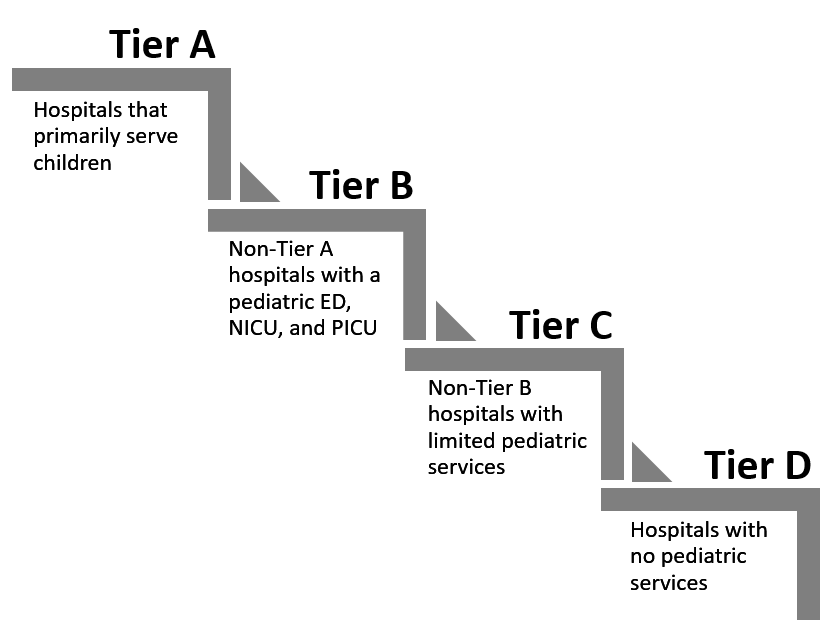
\includegraphics[height=2in, keepaspectratio]{CH-tiers.png}
    \end{figure}
\end{frame}

\begin{frame}{Distribution of Procedures}
    \only<1>{
    \begin{table}[htb!]
    \centering
    \centerline{
    \begin{tabular}{l|rrrrr}
        Surgery & Tier A & Tier B & Tier C & Tier D & Unassigned \\
        \hline\hline
        Circumcision                        & 199 & 217 & 275 & 43 & 17 \\
        Appendectomy                        & 4,136 & 4,519 & 5,627 & 786 & 355 \\
        Posterior spinal fusion             & 1,844 & 1,267 & 454 & 46 & 210 \\
        Repair of humerus fracture          & 800 & 1,038 & 590 & 38 & 66 \\
        Tonsillectomy and adenoidectomy     & 799 & 770 & 363 & 28 & 44 \\
        Tympanostomy                        & 545 & 384 & 92 & & 46 \\
        Orchiopexy                          & 88 & 106 & 81 & & \\
        Umbilical hernia repair             & 82 & 69 & 33 & & \\
        Inguinal hernia repair              & \multicolumn{4}{c}{$<$ 10 patients} \\
        Strabismus surgery                  & \multicolumn{4}{c}{$<$ 10 patients} \\
    \end{tabular}}
    \end{table}
    }
    \only<2>{
    \begin{figure}[htb!]
        \centering
        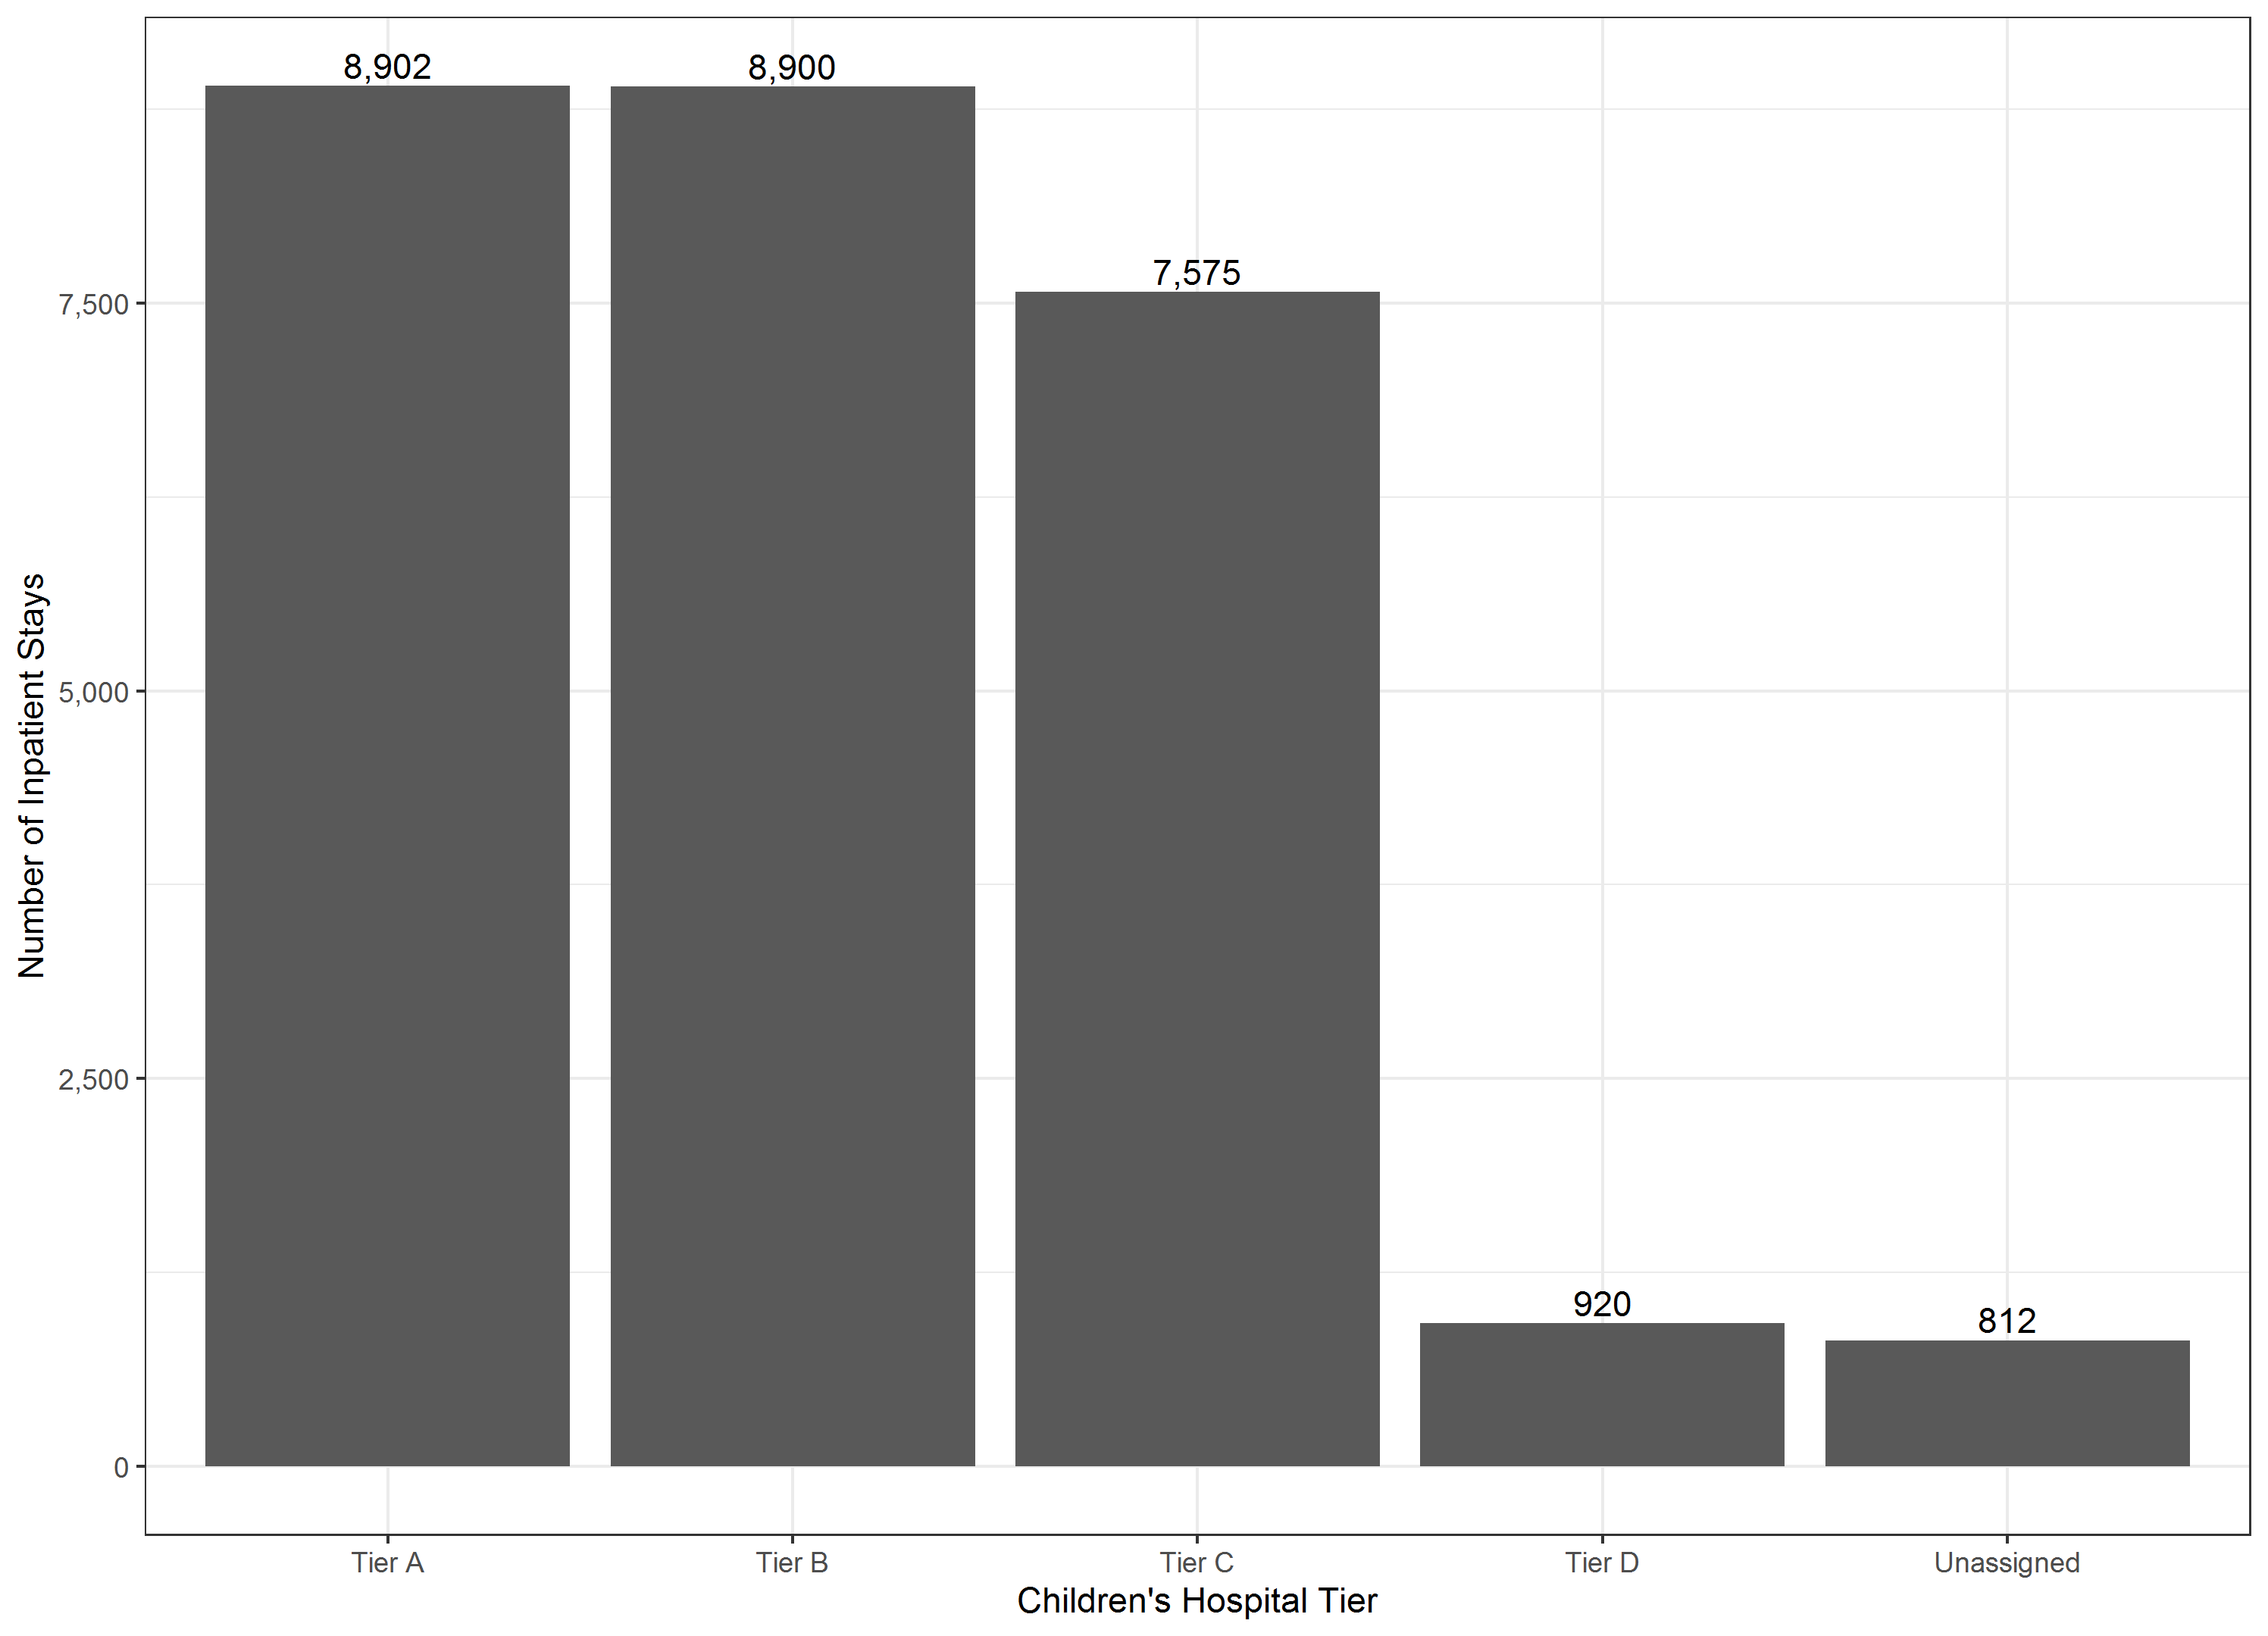
\includegraphics[height=2in]{ch-tiers-nocircum.png}
    \end{figure}
    }
\end{frame}

\begin{frame}{Growth of Children's Hospitals}
\only<1-2>{
    %Number of specialty hospitals
    \begin{center}
    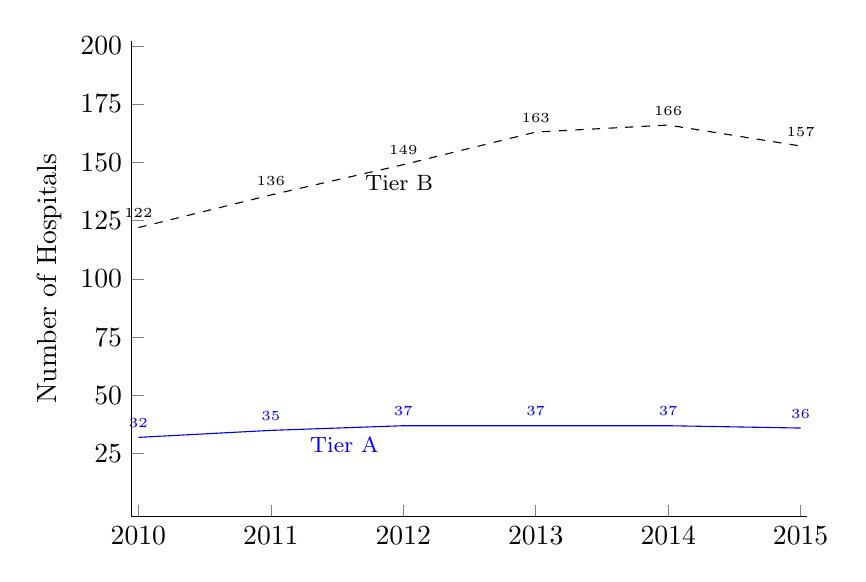
\begin{tikzpicture}
    \pgfmathsetlengthmacro\MajorTickLength{
      \pgfkeysvalueof{/pgfplots/major tick length} * 0.5
    }
    \begin{axis}[
        color=black,
        axis lines*=left,
        width=4in,
        height=3in,
        %bar width=6pt,
        %ybar,
        enlargelimits=0.01,
        ylabel={Number of Hospitals},
        symbolic x coords={2008,2009,2010,2011,2012,2013,2014,2015},
        xtick=data,
        ytick={25, 50, 75, 100, 125, 150, 175, 200},
        ymin=0,
        ymax=200,
        nodes near coords,
        every node near coord/.style={/pgf/number format/precision=3},
        every node near coord/.append style={font=\tiny},
        nodes near coords align={vertical},
        nodes/.style={font=\footnotesize}
    ]
       \addplot[color=blue, thin] coordinates {
        (2010,32)
        (2011,35)
        (2012,37)
        (2013,37)
        (2014,37)
        (2015,36)
        }
        node[midway,below] {\footnotesize{Tier A}}
        ;
       \only<2>{
       \addplot[color=black, dashed] coordinates {
        (2010,122)
        (2011,136)
        (2012,149)
        (2013,163)
        (2014,166)
        (2015,157)
        }
        node[midway,below] {\footnotesize{Tier B}}
        ;
       }
       \end{axis}
    \end{tikzpicture}
    \end{center}
    }
    
    \only<3>{
    \begin{figure}[htb!]
        \centering
        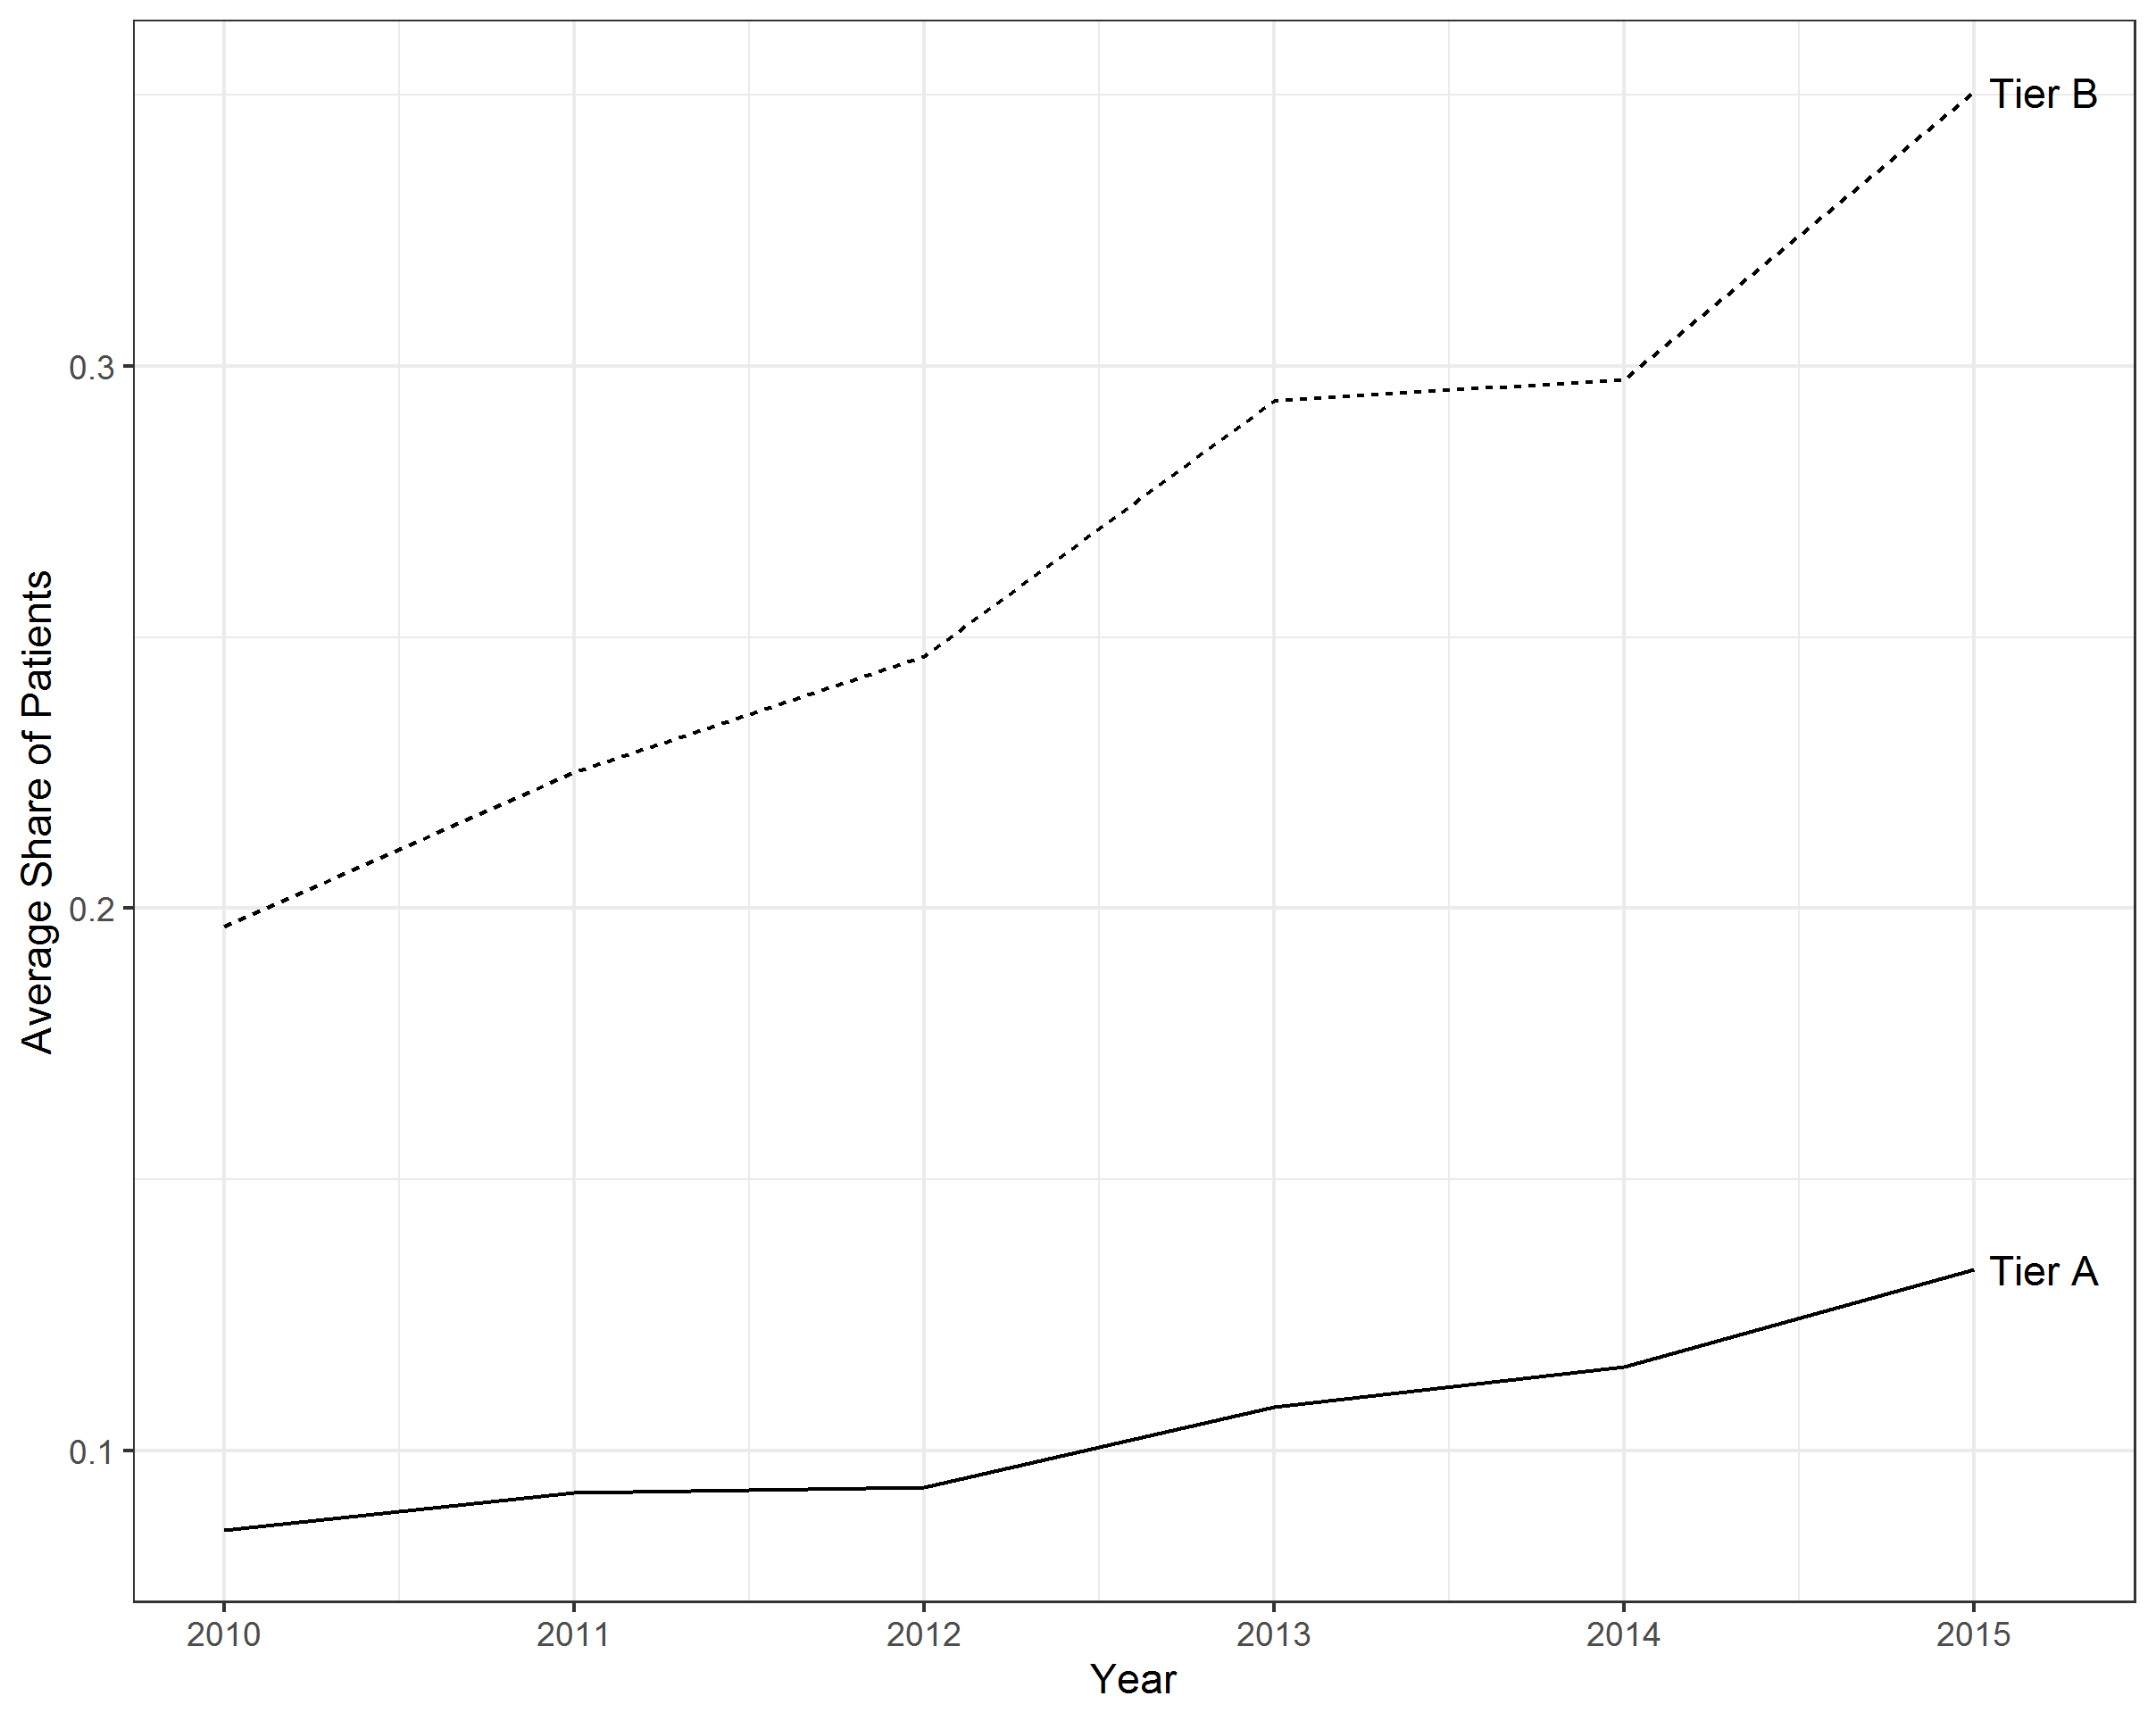
\includegraphics[height=2.5in, keepaspectratio]{tierab-shares-hrr.png}
    \end{figure}
    }
\end{frame}

\section{Are Children's Hospitals More Expensive?}
\begin{frame}{Comparison of Hospitals}
    \begin{table}[htb!]
    \centering
    \centerline{
    \begin{tabular}{l|rrr}
         & Tier A & Tier B & Tier C \\
        \hline\hline
        Price               & \$20,452  & \$13,553  & \$11,863  \\
        Bed Size            & 290       & 665       & 301       \\
        Nonprofit           & 98\%      & 74\%      & 78\%      \\
        Teaching            & 46\%      & 58\%      & 10\%      \\
        System              & 23\%      & 72\%      & 68\%      \\
        Total Discharges    & 11,549    & 31,765    & 14,667    \\
        HCCI Patients       & 42        & 10        & 3         \\
        Complication Rate   & 1\%       & 1\%       & 1\%       \\
        Readmission Rate    & 27\%      & 14\%      & 9\%       \\
        \hline
        Count               & 218       & 903       & 3,068     \\
    \end{tabular}}
    \end{table}
\end{frame}

\begin{frame}{Adjusted Comparison}
    \begin{table}[htb!]
    \centering
    \centerline{
    \begin{tabular}{l|rrr}
         & Tier A & Tier B & Tier C \\
        \hline\hline
        Price               & \$6,788  & \$3,034  & \$2,789  \\
        Complication Rate   & 1\%       & 1\%       & 1\%       \\
        Readmission Rate    & 38\%      & 26\%      & 22\%       \\
        \hline
        Count               & 202       & 522       & 403        \\
    \end{tabular}}
    \end{table}
\end{frame}


\begin{frame}{Price Differentials in Regression Context}
    \begin{table}[htb!]
    \centering
    \centerline{
    \begin{tabular}{l|rrrr}
            &   (1) &   (2) &   (3) &   (4)     \\
\hline\hline
Tier A or B &            1,900***     & 1,300*  & 1,300*       & 1,259*       \\
            &             (713)       &  (746)  &  (751)       &  (752)       \\
Complications &                  &              & -53          &              \\
              &                  &              &  (7,454)     &              \\
Readmission &                    &              &              & 2,083        \\
            &                    &              &              &  (1,464)    \\
\hline
County FE &             Yes      &     Yes      &     Yes      &     Yes      \\
Year FE &               Yes      &     Yes      &     Yes      &     Yes      \\
Hospital Controls &      No      &     Yes      &     Yes      &     Yes      \\
County Controls &        No      &     Yes      &     Yes      &     Yes      \\
Observations &         1,178     &    1,178     &    1,178     &    1,178     \\
    \end{tabular}}
    \end{table}
\end{frame}


\begin{frame}{Complication Differentials in Regression Context}
    \begin{table}[htb!]
    \centering
    \centerline{
    \begin{tabular}{l|rrr}
             &   (1) &   (2) &   (3)     \\
\hline\hline
Tier A or B &                    0.005 &           0.003 &          0.003  \\
            &                    (0.004) &         (0.004) &        (0.004)  \\
Average Price (1000s) &              &                 &       -0.00001  \\
                      &              &                 &       (0.0003)   \\ 
\hline
County FE &             Yes      &     Yes      &     Yes      \\
Year FE &               Yes      &     Yes      &     Yes      \\
Hospital Controls &      No      &     Yes      &     Yes      \\
County Controls &        No      &     Yes      &     Yes      \\
Observations &         1,178     &    1,178     &    1,178     \\
    \end{tabular}}
    \end{table}
\end{frame}


\begin{frame}{Readmission Differentials in Regression Context}
    \begin{table}[htb!]
    \centering
    \centerline{
    \begin{tabular}{l|rrr}
             &   (1) &   (2) &   (3)     \\
\hline\hline
Tier A or B &                    0.05*** &           0.02 &          0.02  \\
            &                    (0.02)  &         (0.02) &        (0.02)  \\
Average Price (1000s) &              &                 &        0.001  \\
                      &              &                 &       (0.003) \\
\hline
County FE &             Yes      &     Yes      &     Yes      \\
Year FE &               Yes      &     Yes      &     Yes      \\
Hospital Controls &      No      &     Yes      &     Yes      \\
County Controls &        No      &     Yes      &     Yes      \\
Observations &         1,178     &    1,178     &    1,178     \\
    \end{tabular}}
    \end{table}
\end{frame}

\section{Willingness to Pay}
\begin{frame}{Hospital Choice Model}
    \textit{Ex post} expected utility: $$u_{ij} = \beta x_{ij} - \gamma p_{ij} + \epsilon_{ij}.$$ 
    \only<2>{
        $x_{ij}$ includes:
        \begin{itemize}
            \item Hospital characteristics (bed size, system, teaching, and for-profit status)
            \item Patient differential distance
            \item Patient characteristics (interactions with gender and length of stay)
        \end{itemize}
    }
    \only<3>{
        $p_{ij}$ denotes predicted out-of-pocket costs for patient $i$ at hospital $j$
    }
    \only<4>{
        Estimate standard multinomial logit model, assuming:
        \begin{itemize}
            \item All hospitals within 90 miles are part of choice set
            \item All hospitals are in network
            \item No outside option...``captive market of patients who must go to one of the hospitals.''
        \end{itemize}
    }
\end{frame}

\begin{frame}{Willingness to Pay}
    \only<1>{
        Expected maximum utility, 
        \begin{align*}
            V_{i} &= \text{E} \max_{j \in J} \left[u\left(x_ij,p_{ij}\right) + \varepsilon_{ij} \right] \\
                  &= \text{ln} \left[\sum_{j \in J} \text{exp}\left(u_{ij}\right) \right]
        \end{align*}
    }
    \only<2>{
        Gain in expected utility from hospital $j$ being in network: $$ \triangle V_{ij} = V_{i}\left(J\right) - V_{i} \left(J \not j \right)$$
    }
    \only<3>{
        Willingness to pay for hospital $j$ to be in network: $$ \triangle W_{ij} = \frac{\triangle V_{ij}}{\hat{\gamma}} $$
    }
    \only<4>{
        In practice:
        \begin{enumerate}
            \item Estimate linear regression of observed prices (allowed amounts) on patient characteristics and surgery indicators
            \item Form predicted prices and predicted out-of-pocket costs from observed \% cost sharing applied to predicted price
            \item Estimate multinomial choice model
            \item Calculate willingness to pay, $\triangle W_{ij}$, for all $i$ and $j$
            \item Sum $\triangle W_{ij}$ across $i$ for each $j$
            \item Average by hospital type (Tier A, Tier B, and Tier C) per year
        \end{enumerate}
    }
\end{frame}

\begin{frame}{Estimated Willingness to Pay}
\only<1-3>{
    %Estimated willingness to pay for CH tier
    \begin{center}
    \begin{tikzpicture}
    \pgfmathsetlengthmacro\MajorTickLength{
      \pgfkeysvalueof{/pgfplots/major tick length} * 0.5
    }
    \begin{axis}[
        color=black,
        axis lines*=left,
        width=4in,
        height=3in,
        %bar width=6pt,
        %ybar,
        enlargelimits=0.01,
        ylabel={Willingness to Pay (\$1000s)},
        symbolic x coords={2010,2011,2012,2013,2014,2015},
        xtick=data,
        ytick={10, 20, 30, 40, 50, 60},
        ymin=0,
        ymax=60,
        nodes near coords,
        every node near coord/.style={/pgf/number format/precision=2},
        every node near coord/.append style={font=\tiny},
        nodes near coords align={vertical},
        nodes/.style={font=\footnotesize}
    ]
       \addplot[color=blue, thin] coordinates {
        (2010,15.60)
        (2011,43.46)
        (2012,29.25)
        (2013,23.21)
        (2014,30.84)
        (2015,53.02)
        }
        node[midway,below] {\footnotesize{Tier A}}
        ;
       \only<2-3>{
       \addplot[color=black, dashed] coordinates {
        (2010,9.44)
        (2011,23.91)
        (2012,13.55)
        (2013,12.73)
        (2014,11.99)
        (2015,15.04)
        }
        node[midway,below] {\footnotesize{Tier B}}
        ;
       }
       \only<3>{
       \addplot[color=red, dotted] coordinates {
        (2010,5.40)
        (2011,16.83)
        (2012,6.06)
        (2013,6.31)
        (2014,5.61)
        (2015,8.46)
        }
        node[midway,below] {\footnotesize{Tier C}}
        ;
       }       
       \end{axis}
    \end{tikzpicture}
    \end{center}
    }
\end{frame}
 
\section{Next Steps}

\begin{frame}{Concerns}
    \begin{itemize}
        \item What is treatment assignment?
        \item Children's and non-children's hospitals are fundamentally different (bed size, for-profit status, etc.)
    \end{itemize}
\end{frame}

\begin{frame}{Move to market level?}
\only<1-3>{
    %Estimated willingness to pay for CH tier
    \begin{center}
    \begin{tikzpicture}
    \pgfmathsetlengthmacro\MajorTickLength{
      \pgfkeysvalueof{/pgfplots/major tick length} * 0.5
    }
    \begin{axis}[
        color=black,
        axis lines*=left,
        width=4in,
        height=3in,
        %bar width=6pt,
        %ybar,
        enlargelimits=0.01,
        ylabel={Count of HRRs},
        symbolic x coords={2010,2011,2012,2013,2014,2015},
        xtick=data,
        ytick={50, 100, 150, 200, 250, 300, 350},
        ymin=0,
        ymax=350,
        nodes near coords,
        every node near coord/.style={/pgf/number format/precision=2},
        every node near coord/.append style={font=\tiny},
        nodes near coords align={vertical},
        nodes/.style={font=\footnotesize}
    ]
       \addplot[color=blue, thin] coordinates {
        (2010,42)
        (2011,44)
        (2012,43)
        (2013,41)
        (2014,38)
        (2015,38)
        }
        node[midway,below] {\footnotesize{Tier A}}
        ;
       \only<2-3>{
       \addplot[color=black, dashed] coordinates {
        (2010,107)
        (2011,109)
        (2012,120)
        (2013,124)
        (2014,131)
        (2015,131)
        }
        node[midway,below] {\footnotesize{Tier B}}
        ;
       }
       \only<3>{
       \addplot[color=red, dotted] coordinates {
        (2010,302)
        (2011,303)
        (2012,300)
        (2013,301)
        (2014,301)
        (2015,300)
        }
        node[midway,below] {\footnotesize{Tier C}}
        ;
       }
       \end{axis}
    \end{tikzpicture}
    \end{center}
    }
\end{frame}


\section*{Thank You}


\end{document}






